\chapter{Large-Scale Graph Processing using Accelerator-Based System}
%\section{Introduction}
The need to rapidly process large graph-structured data, in both scientific and commercial applications, has engendered
recent efforts to leverage cost-efficient GPUs \cite{Rain, Strings} for efficient graph analytics. Doing so, however, requires
addressing substantial technical challenges, including (1) dealing with the dynamic nature of graph parallelism \cite{medusa, mapgraph, cusha, naila}, (2) coping with limited on-GPU memory, i.e., to process graphs with memory footprints
that exceed limited GPU memory sizes \cite{chi, xstream}, and (3) addressing programmability issues for developers with limited
insights into how to best exploit the resources of evolving and varied GPU architectures \cite{ppl,pact,jure}.

Previous work on parallel graph processing has sought to exploit scale-out methods, by distributing
large graph data across the different nodes of computational clusters \cite{graphlab}. Recognizing the low computation to 
communication ratios of typical graph processing algorithms \cite{chi,xstream}, the `GraphReduce' (GR) programming
framework presented in this chapter uses the alternative `scale up' approach in which large graphs processed 
by memory-limited GPUs can take advantage of the potentially considerable memory capacities of the host machines 
to which they are attached. The implementation of GR for NVIDIA GPUs evaluated in this chapter efficiently runs 
irregular graph algorithms on datasets considerably larger than GPU memory sizes, by (i) partitioning graphs into
fixed size chunks -- shards -- asynchronously moved between GPU and host, (ii) adopting a combination of 
of edge-(X-Stream \cite{xstream}) and vertex-(GraphChi \cite{chi}) centric implementations of graph representations,
(iii) overlapping GPU computation with data transfer via concurrent GPU operations, using CUDA streams, and 
(iv) using `spray' operations to further divide shards and obtain fine-grain parallelism that exploits the 
Hyper-Q feature of Kepler GPUs \cite{kepler}. Specifically, spray operations are used to further divide each shard into multiple 
sub-buffers transferred over dynamically created CUDA streams. The purpose is efficiently use GPU hardware features
like Hyper-Qs.

GraphReduce runs graph algorithms on GPUs without unduly burdening graph algorithm developers. 
Programmers write the appropriate sequential codes for their algorithms, e.g., for data mining, machine learning, etc.,
and then use its simple API to express their use for processing entire graphs. The GR runtime partitions the
graph into different shards, each single one of which entirely fits into GPU memory. Graph processing, then, 
overlaps shard movement with GPU-level graph processing, the latter using multiple levels of GPU-level parallelism,
as indicated above. With such automation, GR can deal with graph sizes much exceeding GPU memory sizes. This is
important because even a common Yahoo web-graph comprised of 1.4 billion vertices \cite{yahoo} requires approximately 
6.6 GB of memory to store just its vertex values (not even including the edges and their status). 

In summary, with GraphReduce, GPUs can be used to accelerate analytics performed on graphs with billions of edges, 
operating at speeds much exceeding that of similar operations run on CPUs, and programmed in ways accessible 
to programmers who are not experts in GPU programming. To the best of our knowledge, GraphReduce is the first
to support in-GPU-memory and out-of-GPU-memory graph processing, thus aiming for scale-up graph processing 
on HPC systems with discrete GPUs and high end (i.e., memory-rich) hosts.

\section{Background and Motivation}
\label{bg}

This section introduces the computational model used in GraphReduce. It also motivates the GR approach by describing some of
the challenges faced by the existing state-of-the-art graph processing approaches.

%\vspace{-0.5\baselineskip}

\subsection{Computational Model: GAS Abstraction}


\begin{figure}[!t]
\centering
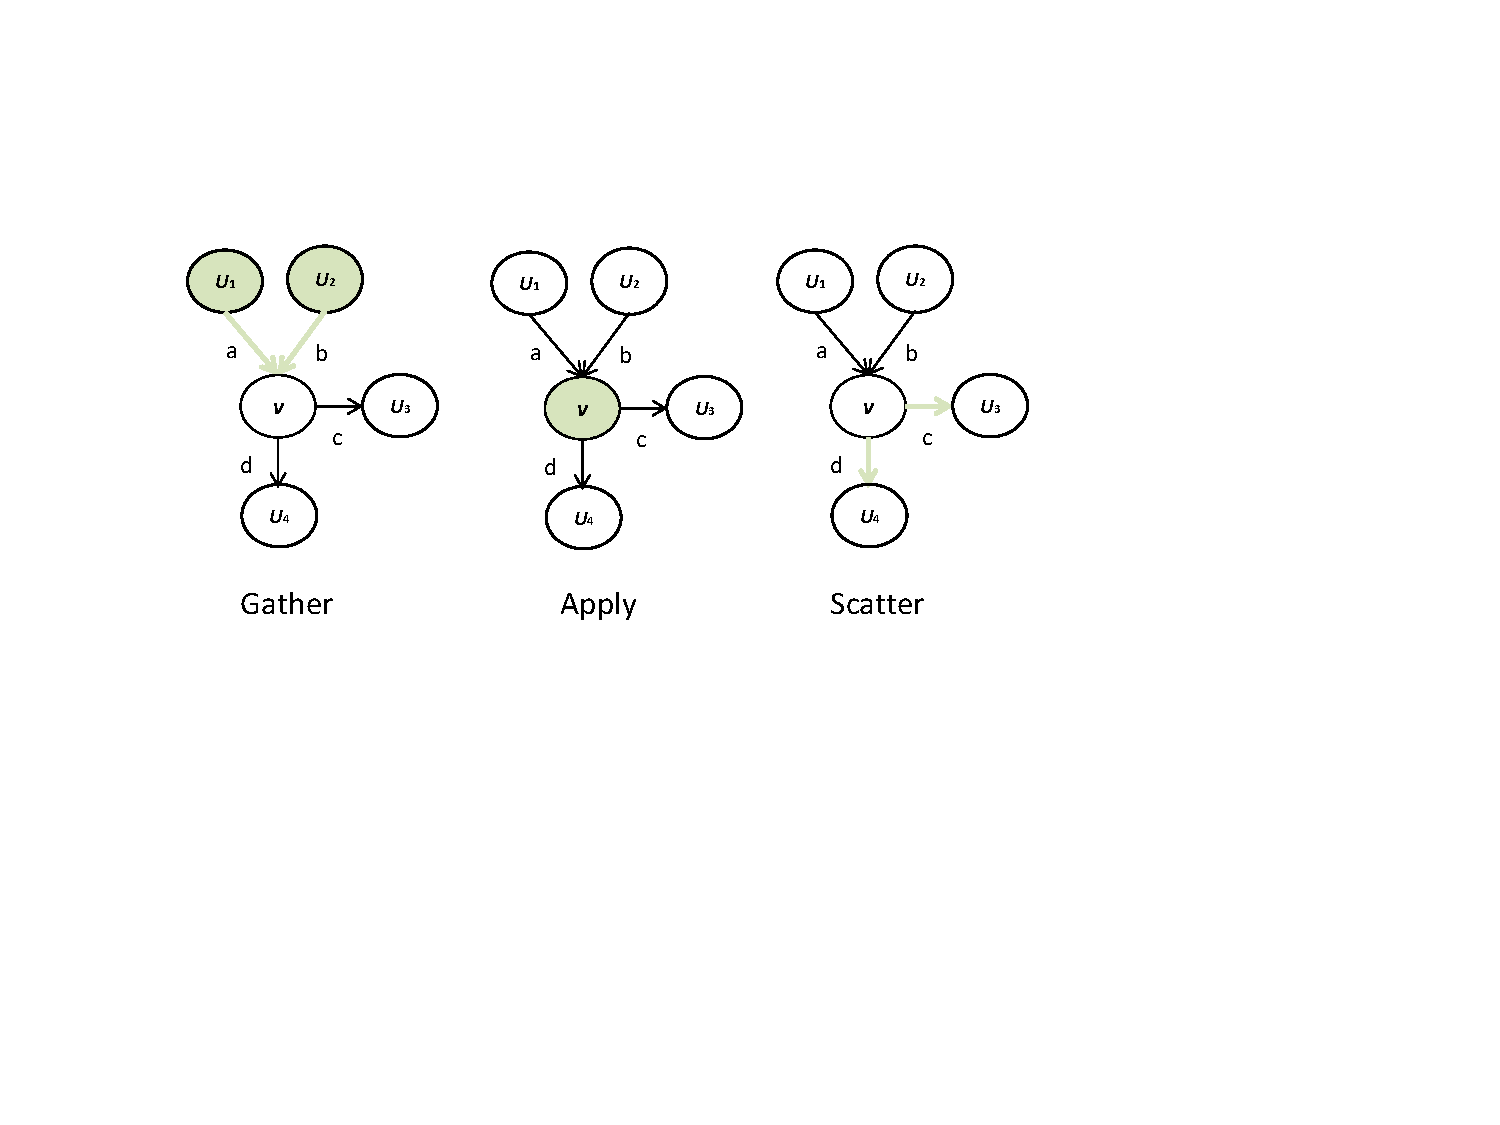
\includegraphics[width=0.9\textwidth,height=\textheight,keepaspectratio]{figures/phases.pdf}
\caption{An example of GAS abstraction. }
\label{fig:phases}
%\vspace{-1\baselineskip}
\end{figure}


GraphReduce exposes the Gather-Apply-Scatter (GAS) computational model used by Pregel \cite{pregel}, Powergraph \cite{powergraph}, and GraphLab \cite{graphlab}.
With GAS, a problem is described as a directed (sparse) graph, $G = (V, E)$, where $V$ denotes the vertex set and $E$ denotes 
the directed edge set. A value is associated with each vertex $v\in V$, and each directed edge $e_{ij}$ is associated with 
a source vertex $u$ and a target vertex $v$: $e_{ij} =(u, v) \in E$. Given a directed edge $e_{ij} = (u, v)$, we refer to 
$e_{ij}$ as vertex $v$'s in-edge, and as vertex $u$'s out-edge. A typical GAS computation, then, has three stages \cite{vertexapi}: 
(1) Initialization, (2) Iterations, and (3) Output. Initialization deals with initializing vertex/edge values and a starting 
{\em computation frontier}, which is defined as the set of active vertices for a given iteration. In each Iteration stage, 
a sequence of iterations is run, each gathering the values seen on the incoming edges, updating the values of elements, and 
then defining a new frontier for the next iteration. Figure \ref{fig:phases} illustrates these three phases, assuming vertex $v$ to be the 
central vertex.


%\vspace{-0.5\baselineskip}
\begin{itemize}
  \item {\bf Gather Phase}: each vertex aggregates values associated with its incoming edges and their source vertices. 
We define the gather function as $G(u, v, e_{ij})$, and we use binary operator $\biguplus$ to aggregate the outputs 
from multiple $G$s into one value $R$. In Figure 1 (a), the result ($R$) from the Gather Phase for vertex $v$ can be represented 
as $R= G(u_1, v, a)\biguplus G(u_2, v, b)$. 
 % \vspace{-0.5\baselineskip}
  \item {\bf Apply Phase}: the value of each vertex in the current frontier is updated through the gather result. 
We define the update function as $U(v, R)$, where $R$ is the result from the Gather Phase. Shown in the Figure 1 (b), 
we have the updated vertex $v$ as: $v' = U(v, R)$.  
 % \vspace{-0.5\baselineskip}
  \item {\bf Scatter Phase}: the new vertex state is propagated to neighbors, by updating the state of its out-edges 
(e.g., $c$ and $d$ in Figure 1). We define the Scatter function for updating the out-edges of $v$ as $S(v', e_{out})$, 
where $v'$ is the updated vertex $v$ and $e_{out}$ represents $v$'s out-edges. Shown in Figure 1 (c), two updated edges 
$c'$ and $d'$ are denoted as: $c' = S(v', c)$ and $d' = S(v', d)$.
%\vspace{-0.5\baselineskip}
\end{itemize} 


As shown in much prior work \cite{powergraph, pregel, sc05}, the GAS model is not only simple to use, but it is also sufficiently general to express
a broad set of graph algorithms, ranging from PageRank to Connected Components, and from Heat Simulation to Sparse Linear Algebra. 
For example, the PageRank algorithm \cite{pagerank} can be expressed as follows. In the {\bf Gather Phase}, each vertex $v_i$ in the current 
frontier accumulates $G_i = \sum_{}^{}{\frac{R_j}{n_j}}$ from all in-edges from source vertex $v_j$, where $R_j$ is the rank of 
$v_j$ and $n_j$ is the number of out-edges ($v_j\rightarrow v_i$) of $v_j$. Then, in the {\bf Apply Phase}, vertex $v_i$ updates 
its value using some common PageRank formula like $R_i = 0.85+0.15\times G_i$. Since in PageRank, the values of out-edges of 	$v_i$ will not change 
in the {\bf Scatter Phase}, there are no operations for this phase. 


\begin{figure}[!t]
\centering
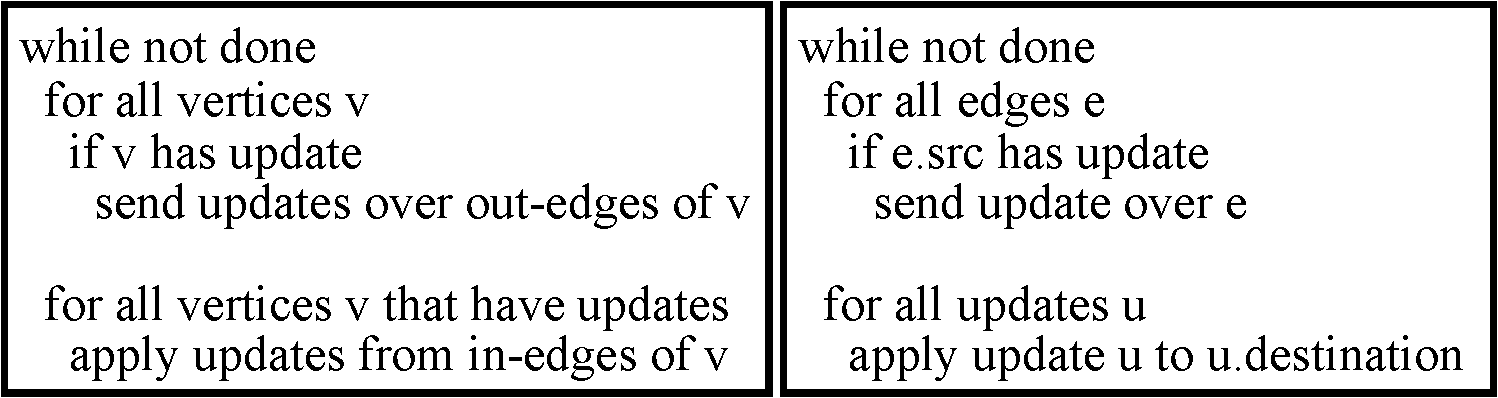
\includegraphics[width=\textwidth,height=\textheight,keepaspectratio]{figures/hybrid-model.pdf}
\caption{ (a) Vertex-centric Scatter-Gather. (b) Edge-centric Scatter-Gather. }
\label{fig:vertex-edge}
%\vspace{-1\baselineskip}
\end{figure}




Figure \ref{fig:vertex-edge} shows two common ways to implement graph algorithms with GAS: edge-centric vs. vertex-centric execution, which differs in whether the
Scatter and Gather phases iterate over and update edges or vertices (their pseudo codes are shown in Figure \ref{fig:vertex-edge}).
Implementation can also vary in terms of Update functions, to be implemented as either Bulk-Synchronous Parallel (BSP) \cite{BSP}
for simplicity or via asynchronous execution, for faster convergence. In either case, the graph algorithm terminates
when some application-specific condition is met, e.g., when no more changes in vertex and edge states beyond a certain threshold. 


\subsection{Motivation and Challenges}

\begin{table}[h]%\scriptsize
\centering
\begin{tabular}{lllc}
Graph Name & Vertices & Edges & \multicolumn{1}{l}{In-memory Size} \\ \hline
\multicolumn{4}{c}{GPU In-Memory} \\ \hline
ak2010\cite{ak2010}& 45,292 & 108,549 & 7.9MB \\
coAuthorsDBLP\cite{coauthors} & 299,067 & 977,676 & 69.5MB \\
kron\_g500-logn20\cite{kron20} & 1,048,576 & 44,620,272 & 2.4GB \\
webbase-1M\cite{web} & 1,000,005 & 3,105,536 & 211.6MB \\
belgium\_osm\cite{belgium} & 1,441,295 & 1,549,970 & 5.4MB \\ \hline
\multicolumn{4}{c}{GPU Out-of-Memory} \\ \hline
kron\_g500-logn21\cite{kron20} & 2,097,152 & 91,042,010 & 4.84GB \\
nlpkkt160\cite{nlpktt} & 8,345,600 & 221,172,512 & 11.9GB \\
uk-2002\cite{uk2002} & 18,520,486 & 298,113,762 & 16.4GB \\
orkut\cite{orkut}& 3,072,441 & 117,185,083 & 6.2GB \\
cage15\cite{cage15} & 5,154,859 & 99,199,551 & 5.4GB
\end{tabular}
\caption{ Datasets used to evaluate GraphReduce framework. `Out-of-memory' means that the input graphs cannot fit into the limited GPU memory. A commercial K20c GPU with a 4.8 GB global memory is used as an example to illustrate in-memory and out-of-memory cases.}
\label{datasets}
%\vspace{-0.5\baselineskip}
\end{table}




\begin{table}[h]%\scriptsize
\centering
\begin{tabular}{cccc}
\hline
Graphs & X-Stream (ms) & CuSha(ms) & \multicolumn{1}{l}{Speedup} \\ \hline
ak2010 & 215.155 & 7.75 & 28x \\
belgium\_osm & 2695.88 & 791.299 & 3x \\
coAuthorsDBLP & 1275 & 11.553 & 110x \\
delaunay\_n13 & 80.89 & 5.184 & 16x \\
kron\_g500-logn20 & 46550.7 & 119.824 & 389x \\
webbase-1M & 3909.12 & 13.515 & 290x
\end{tabular}
\caption{Performance comparision between two state-of-the-art graph processing approaches. X-Stream runs on a 16 core Xeon E5-2670 CPU with 32GB memory. CuSha runs on a NVIDIA K20c Kepler GPU with 4.8 GB memory. }
\label{gpu-cpu}
%\vspace{-0.5\baselineskip}
\end{table}


\subsubsection{Why Graph Analytics Using GPUs ?}
The high compute power and multi-level parallelism provided by the SIMT (Single Instruction Multiple Threads) architectures of GPGPUs \footnote{\scriptsize Without specified mention, NVIDIA terminology will be used throughout the chapter
to illustrate our work. However, the proposed methodology can be easily applied to a wide range of massively
parallel architectures.} present opportunities for 
accelerating many graph algorithms \cite{medusa, cusha,vertexapi,mapgraph}. Table \ref{gpu-cpu} shows the performance comparison between two state-of-the-art graph analytics 
processing the BFS algorithm: X-Stream \cite{xstream} for CPUs and CuSha \cite{cusha} for in-memory GPU processing. Significant performance speedups are
observed from using the GPU. For instance,  graph kron\_g500-logn20 \cite{kron20} processed by CuSha on a commercial K20c Kepler GPU 
(4.8GB memory) achieves 390x speedup over X-Stream on a 16 core Xeon E5-2670 CPU (32 GB memory).


\subsubsection{Challenges in GPU Graph Analytics?}
Acceleration of graph analytics via GPUs is limited, however, by the fact that many real-world graphs cannot fit into 
GPUs' limited memories. As mentioned earlier, a common Yahoo-web graph \cite{yahoo} with 1.4 billion vertices requires 6.6 GB memory 
just to store its vertex values. Additional examples of graphs exceeding GPU memory sizes appear in Table \ref{datasets}.
Previous work on GPU-based graph processing has not addressed this issue. CuSha \cite{cusha}, MapGraph \cite{mapgraph}, VertexAPI \cite{vertexapi} and Medusa \cite{medusa} all assume graphs to reside in GPU memory. GraphChi \cite{chi} and X-Stream \cite{xstream} are designed for CPU-based systems, 
unable to benefit from the multi-level massive parallelism offered by GPUs (shown in Table \ref{gpu-cpu}). Hybrid approaches (CPU+GPU) like Totem \cite{totem} are only able to process a fixed sub-graph that can fit into GPU memory after statically partitioning the graph between CPU and GPU, which results in underutilization of GPU's fullest processing power and parallelism. 
 


%Totem \cite{totem} provides a high-level abstraction to address a hybrid environment (CPU+GPUs), 
%by statically partitioning the graphs into GPU and host CPU memories. Specifically, performance improvements are obtained for
%graphs following a power-law vertex distribution by placing low-degree vertices on the CPU and high-degree vertices on the GPU.
%As graph size increases, however, only a fixed sub-graph can fit into GPU memory, leading to diminishing returns for
%such static partitioning, since more and more of the graph processing will be bottlenecked by the slower compute engine (CPU). 




% (\textcolor{red}{/*Figure XX shows examples of large graphs that do not fit in GPU memory and their vertex distributions are not suitable for Totem. I have two graphs of vetex degree %distribution for two large graphs. wait for totem results before adding here /*}). 


\begin{figure}[!t]
\centering
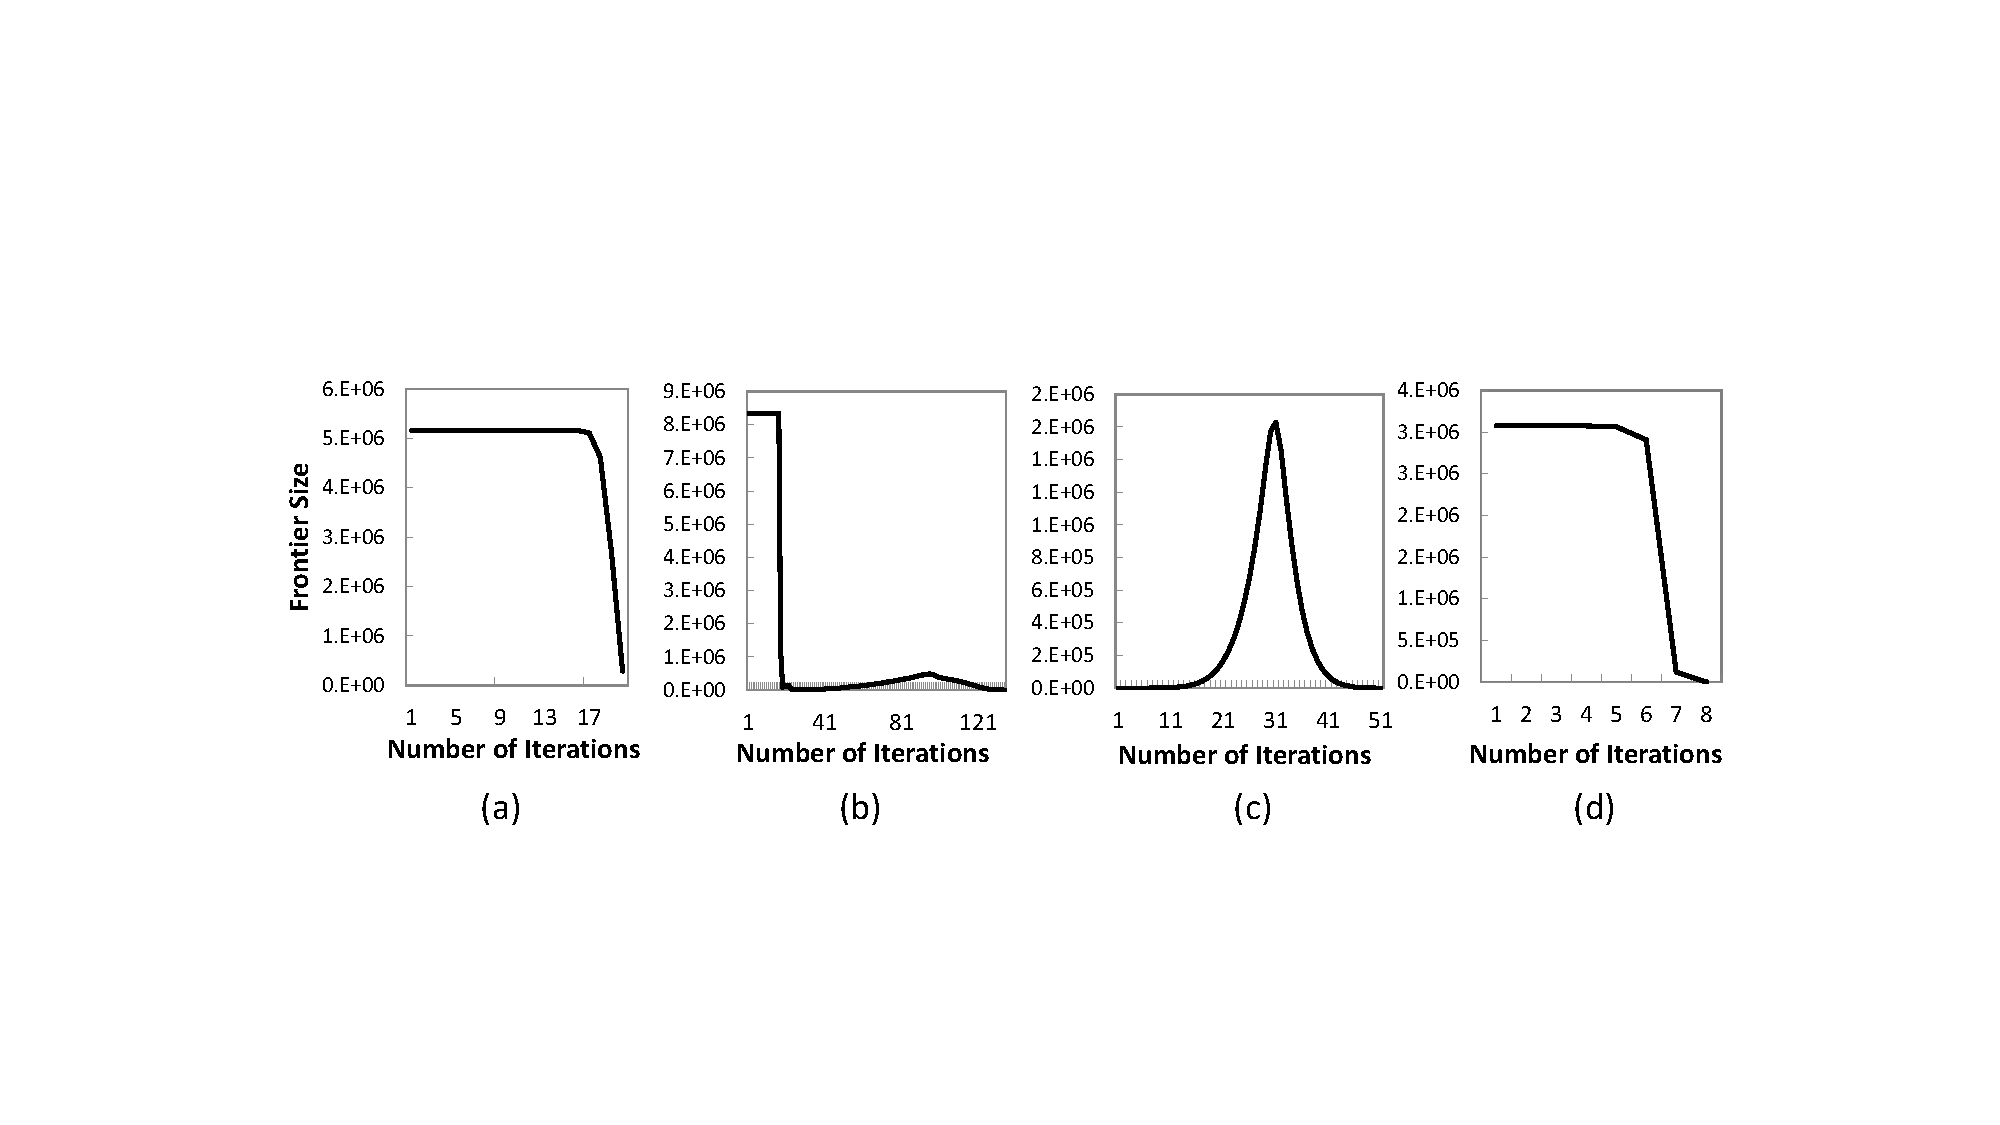
\includegraphics[width=\textwidth,height=\textheight,keepaspectratio]	{figures/frontier.pdf}
\caption{Frontier size changes across iterations using the GAS model on GPUs. This phenomenon highly depends on the input graph and algorithm, showcasing the inherent graph irregularity. Four cases from left to right: (a) Cage15 - PageRank; (b) nlpkkt160 - PageRank; (c) Cage15 - BFS; and (d) orkut - Connected Component (CC). 
 }
\label{fig:frontier}
%\vspace{-0.5\baselineskip}
\end{figure}

\subsubsection{Challenges in Evolving Graph Analytics On GPU}

\begin{figure}[!t]
\centering
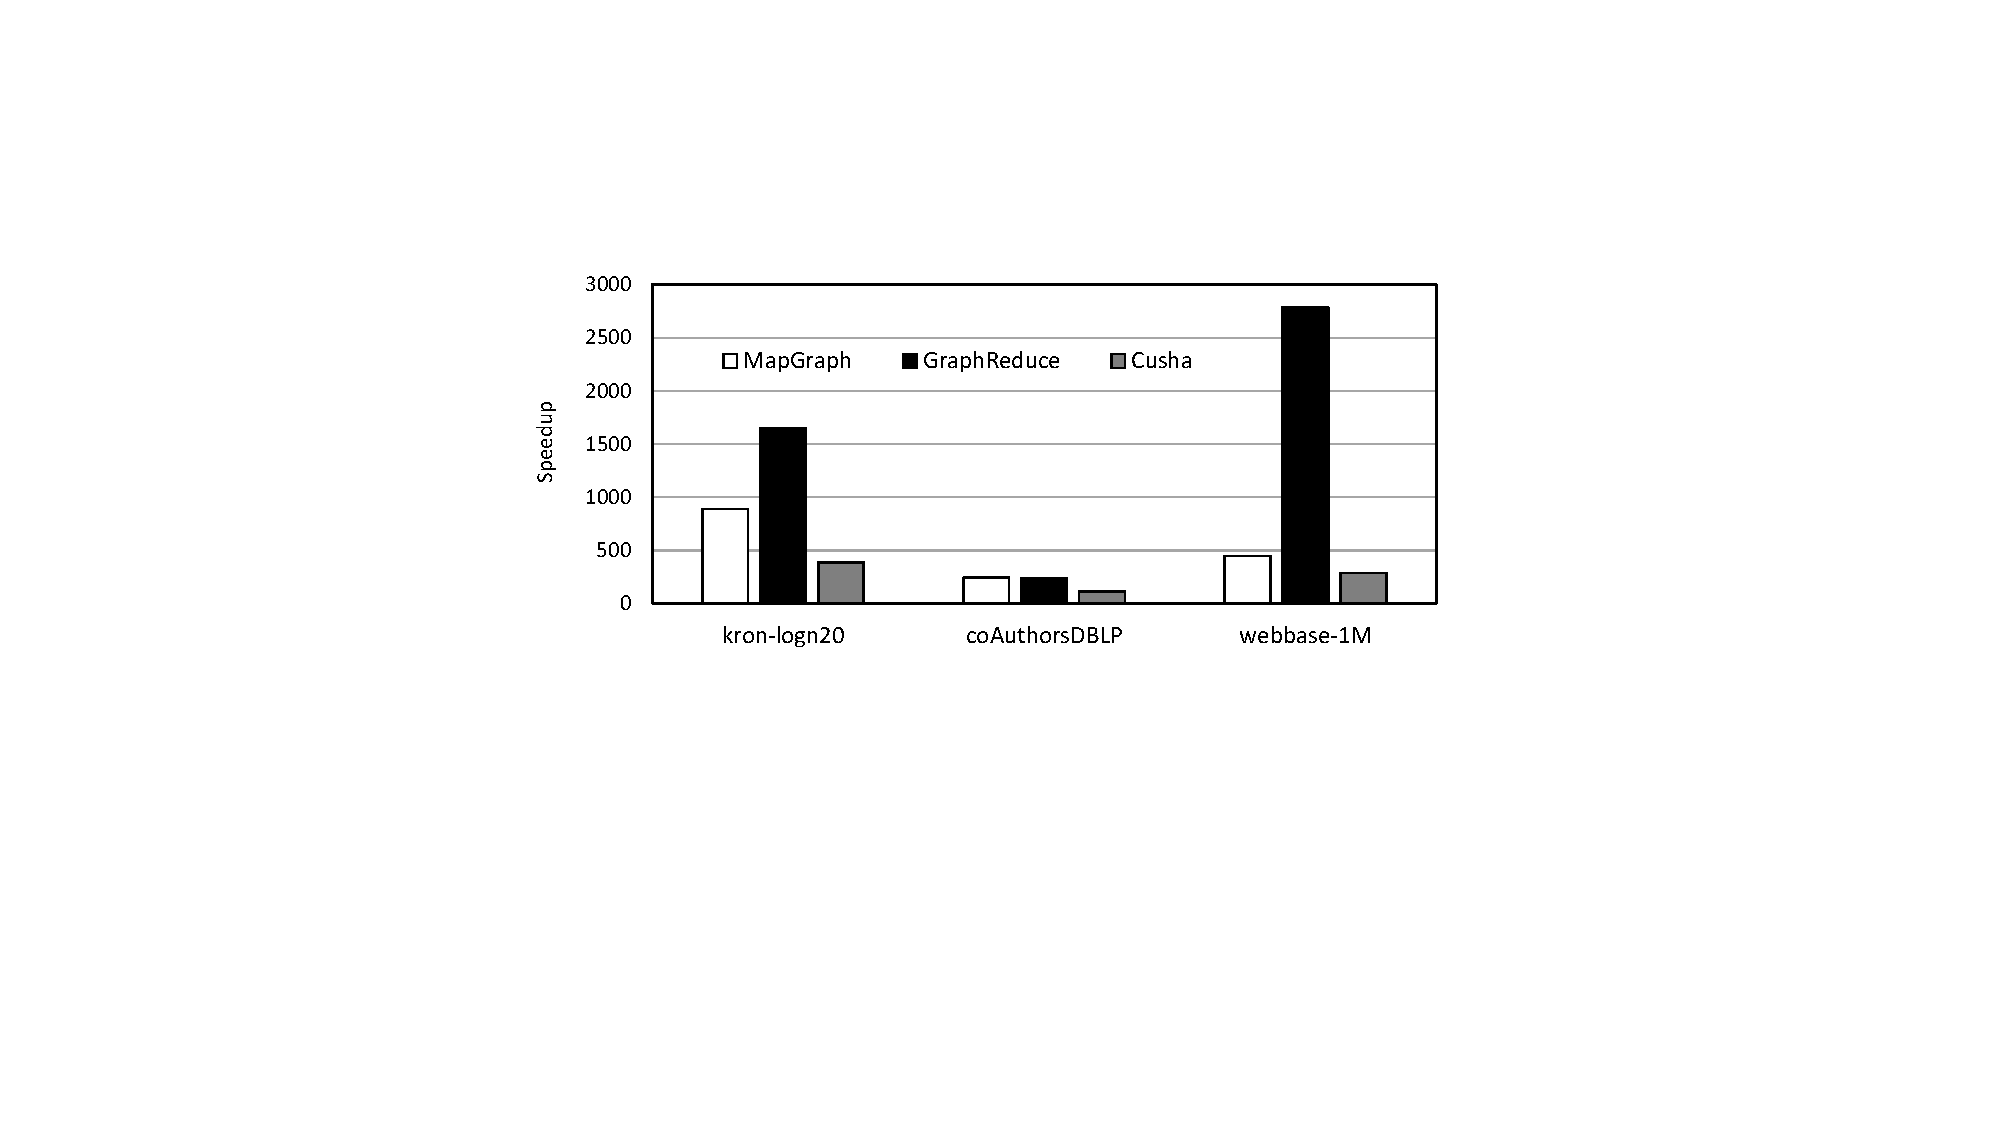
\includegraphics[width=0.75\textwidth,height=0.75\textheight,keepaspectratio]{figures/static_GR.pdf}
\caption{State-of-the-art GPU frameworks (i.e., MapGraph, GraphReduce and Cusha) for processing static graphs significantly outperform the best CPU-based framework X-Stream (baseline).}
\label{fig:static}
%\vspace{-0.5\baselineskip}
\end{figure}

GPUs have emerged as one of the most powerful computation accelerators for world-class supercomputers~\cite{titan} because of their unparalleled massive amount of parallelism and ability to speedup a wide range of HPC applications. Compared to its counterpart CPU, it also often provides superior acceleration for general graph algorithms. Figure \ref{fig:static} demonstrates that for processing three real-wold in-memory \textit{static graphs} under BFS, state-of-the-art GPU frameworks outperform the best CPU-based graph analytics (i.e., X-Stream) by an average speedup of 782x and up to 2785x (i.e., GraphReduce on \textit{webbase-1M}). This motivates us to unleash GPU's high computation power for processing \textit{evolving dynamic graphs}. 

Figure \ref{fig:link} shows an example of an evolving Linkedin social network graph, in which a subgraph (circled by red dashed line) is going through \textit{update batches} (e.g., insert:(1,4) and delete:(1,3)) at different time point. Different colors of dots represent work fields. Processing such common constantly-evolving social network graphs on GPUs is very challenging because (i) highly efficient computation model and convenient programming constructs do not exist for programmers to effectively express their algorithms on GPUs, (ii) how to efficiently utilize the parallelism provided by GPUs to deal with the computation and data storage overlap in dynamic graphs is complicated, and (iii) how to extract the most throughput from GPUs without burdening the users with hardware details is unclear. In order to address these challenges, we designed a runtime graph analytics framework named \textit{EvoGraph} to process complex evolving graphs on modern GPUs. Under EvoGraph, users only need to write sequential codes and the sophisticated runtime will seamlessly map the incremental graphs to GPU for acceleration. We will discuss the design details of EvoGraph next. 



\begin{figure}[!t]
%\vskip -3 mm
\centering
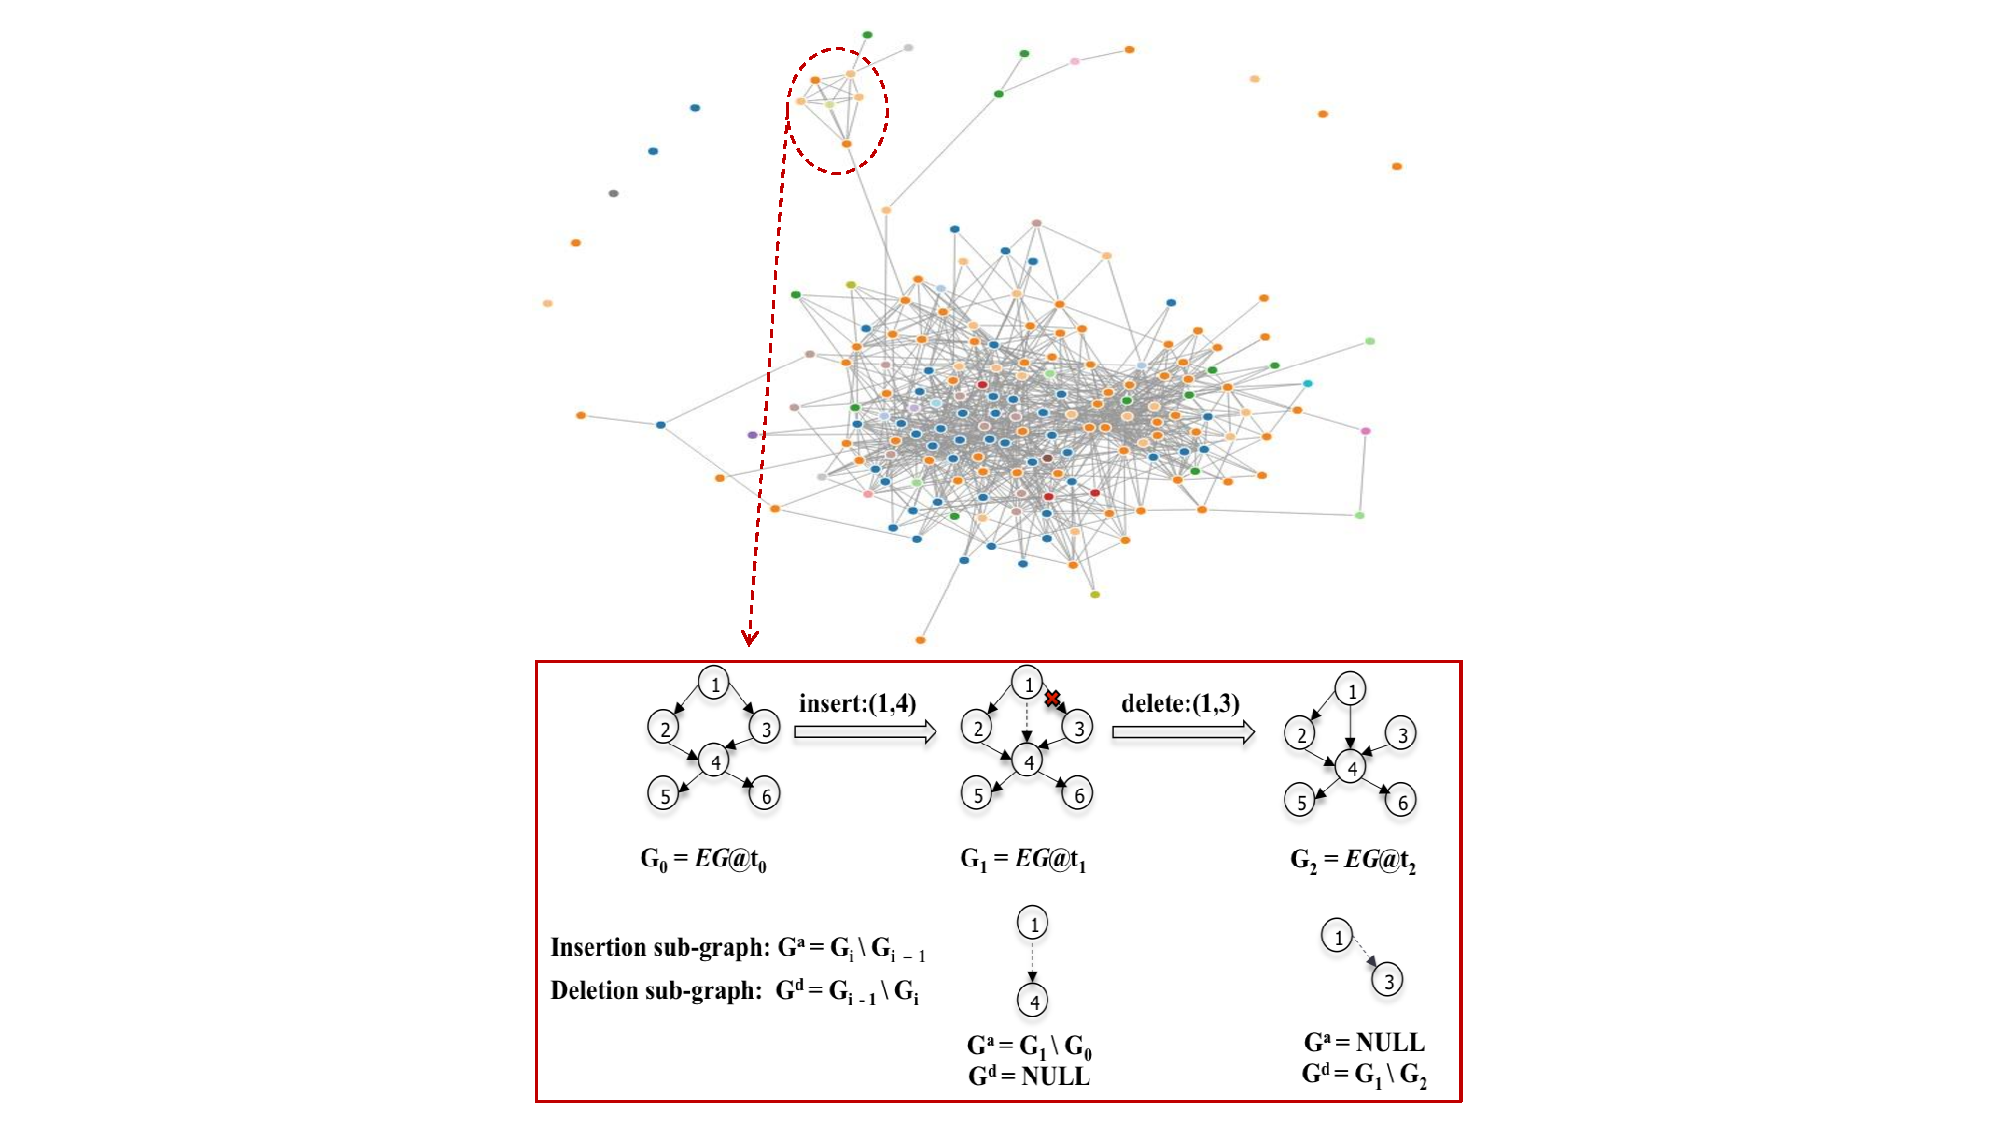
\includegraphics [width=1\columnwidth]{figures/link.pdf}
\caption{A subgraph of a Linkedin social network has been updated over time but the rest of the network remains the same. }
\label{fig:link}
%\vspace{-0.5\baselineskip}
%\vskip -3 mm
\end{figure}



There are several challenges to efficiently process larger-than-memory graphs on GPUs. They involve the need to provide end
users with convenient programming constructs for their graph algorithms, but without unduly burdening them with (i) graph partitioning to
fit sub-graphs into GPU memory, (ii) how and when such partitions are moved between GPU and host memories, and (iii) how to best
extract multi-level parallelism from their GPU-resident execution. The GraphReduce framework presented in this chapter 
addresses these challenges.




Graph partitioning or chunking for fitting into GPU memory must deal with the irregular nature of 
graph algorithms and how they access the input data. More specifically, to obtain high on-GPU performance, chunking
must be done to minimize GPU-host data movement. For the GAS model, this requires ensuring GPU memory residence of 
the vertices and edges that actively take part in the computation iterations being performed.
This despite the fact that due to the inherent irregularity in graph algorithms, in every computation iteration, the number 
of edges and vertices that actively take part in computation (computation frontier size) is not constant, and it varies with 
graph algorithms and datasets, as shown in Figure \ref{fig:frontier}. Across all of these cases, the frontier sizes \footnote{\scriptsize The term ``frontier size" is synonymous with the number of active vertices in a given iteration. The variation of the frontier size during execution is sensitive to the starting-point for graph processing. } 
incur significant changes (either dropping or climbing). For instance, in Figure \ref{fig:frontier}(b) for graph nlpkkt160 processed 
by PageRank, the frontier size drops sharply after a few iterations and remains low for the rest of the execution. 
Given these results, ideally, the GR runtime should {\em move sub-graphs to the GPU only if they
contain active vertices and edges}. Otherwise, such movements simply cause unnecessary overhead.
For the same nlpkkt160 case in Figure \ref{fig:frontier}(b), after several iterations, most of the sub-graphs do not have 
active vertices/edges, so there is no need to move those chunks to the GPU. We have found this phenomena to be very common 
across most of the graphs shown in Table \ref{datasets}, for various algorithms. The GR methods presented in this chapter address this issue, along with (ii) and (iii) above.

%EvoGraph
High performance machines are increasingly using GPUs~\cite{15, 16, 17, 18, 19}, to leverage their scalability and low dollar to FLOPS ratios.  As a result, GPUs have become the main compute engines for today’s HPC clusters and supercomputers like Titan in Oak Ridge~\cite{titan}. This trend continues with the move toward exascale machines that are expected to be comprised of millions of accelerator and general purpose cores, whether packaged as `thin' or `fat' nodes. Another recent trend is the gain in popularity of GPU processing in many domains such as social networks, e-commerce, advertising, and genomics. This has motivated the growing interest in large-scale real-world graph processing for both scientific and commercial applications, as well as the recent efforts in accelerator-based graph processing frameworks such as MapGraph~\cite{mapgraph}, Medusa~\cite{medusa}, CuSha~\cite{cusha}, GraphReduce~\cite{GraphReduce}, and so on. An important aspect of real-world graphs, like Facebook friend lists or Twitter follower graphs, is that they are dynamic.  Given the billions of Facebook~\cite{linkbench} users sharing more than 100 billion photos and posts per month, let alone the volume on Twitter~\cite{twitter} or other blogging platforms, there is a huge need to quickly analyze this high velocity stream of graph data. 

However, state-of-the-art graph analytics for dynamic graphs follow a store-and-static-compute model that involves batching these updates into discrete time intervals, applying all of the updates to the total graph, and then rerunning the static analysis.  There is considerable redundancy and inefficiency in this approach to analyzing this \textit{evolving} graph sequence.  Static graph analytics on a single version of the evolving graph, even when leveraging massive amount of parallelism offered by thousands of cores in a GPU, can be very slow due to the extreme scale of many real-world graphs (e.g., one Facebook graph purportedly has a trillion edges~\cite{fb}) and/or because of the complexity of the graph queries that are traditionally both compute and memory intensive. Second, data movement of the entire input graph repeatedly between the host and the GPU over the slow PCIe link can result in substantial overhead, which in turn can overshadow the benefits from the massive parallelism offered by a GPU.  Finally, there are real world graph analytics problems that inherently require soft or hard real-time guarantees, e.g., real-time anomaly detection, disease spreading, etc, and hence can't use the traditional static recomputation model. Beyond just hardware performance, we also note that the skills to write performant GPU code are substantially different from the coding skills that many analysts have learned.  As one can therefore see, the many demands of high velocity graph data, both commercial and scientific, have outstripped the traditional, batched static graph analytics models, even when using GPUs.

To address this, we propose a two-pronged approach to deal with both the performance and programmability challenges. We introduce an accelerator-based incremental graph processing framework called EvoGraph. EvoGraph employs a new variant of  the popular Gather-Apply-Scatter (GAS) programming model, which we call Incremental-GAS (or I-GAS), to incrementally process a batched stream of updates (i.e., edge/vertex insertions and deletions).  The key insight is that I-GAS algorithms are designed to work over a (dynamically determined) sub-graph of the previous version of the evolving graph.  For many popular graph algorithms and real-world graphs, the corresponding I-GAS logic affects only a fractional portion of the graph; this reduction in problem size can result in tremendous performance benefits compared to static recomputation of the graph algorithm on the entire graph.  The modest additions of the I-GAS model to the already-published GAS model interface enable an easy transition of analysts from coding in a static to a dynamic streaming environment.

From a simplistic view, it would seem that incremental methods would always be preferable.  However, there are scenarios when a streamed update may affect a very large portion of the graph, and incremental processing won't help much or may even be worse than static recomputation due to overheads of incremental execution. One such counterexample is in the incremental version of Breadth First Search (BFS), where updates that affect vertices close to the source/root node will affect nearly the entire BFS tree. Here the incremental run can at best perform as good as the static re-run, and may even be worse. Note that this is not a concern about correctness of the result, but over performance.  Therefore, in order to handle such scenarios, we employ a \textit{per batch}, property-based dynamic choice between incremental and static graph processing called \textit{‘property-guard’}. Utilizing user-defined and built-in properties (e.g., vertex degree) along with programmable control policies, EvoGraph analyzes each update batch and dynamically decides whether to process the graph incrementally using I-GAS or to fall back to static recomputation. 

%\section{Background And Motivation}


%Related Work
\section{Related Work}

{\bf In-Memory Graph Processing.} Merrill \textit{et al.}\cite{Merrill} present 
a parallelization of BFS tailored to the GPU's requirement for large amounts of fine-grained BSP; they achieve an asymptotically 
optimal $O(|V|+|E|)$ work complexity. 
Hong \textit{et al.}\cite{Hong} propose warp-level load-balancing that defers outliers 
and performs dynamic workload distribution to speed up graph algorithms through heavyweight atomic operations on global memory. 
Duong \textit{et al.} \cite{Duong} conduct detailed GPU-based optimizations for PageRank and achieves significant speedup over 
a multi-core CPU implementation. Chapuis \textit{et al.} \cite{ASSP} provide an algorithmic optimization solution to speedup 
all-pairs shortestpath (APSP) for planar graphs that exploits the massive on-chip parallelism available on GPUs. 
GraphReduce can be extended to implement the algorithm-specific optimizations above and in contrast to such work, it offers
user-level APIs for programming graph algorithms and provides a general framework addressing a wide range of parallel graph algorithms 
and hiding architecture-level optimizations from users.

Concerning frameworks for GPU-based graph processing, earlier work like \textit{Medusha} \cite{medusa} introduces some basic
graph-centric optimizations for GPUs, offering a small set of user-defined APIs, but its performance is not comparable to the
state-of-the-art low-level GPU optimizations. To address this issue, \textit{MapGraph} \cite{mapgraph} and \textit{VertexAPI}\cite{vertexapi}
implement runtime-based programming frameworks with levels of performance that match those seen for low-level specific algorithm optimizations. 
\textit{MapGraph} chooses among different scheduling strategies, depending on the size of the frontier and the adjacency lists 
for the vertices in the frontier. 
It also uses a Structure Of Arrays (SOA) pattern to ensure coalesced memory access. 
\textit{VertexAPI} provides a GAS model-based GPU library, gaining high performance primarily from using the 
ModernGPU \cite{moderngpu} library for load balancing and memory coalescing. \textit{CuSha} \cite{cusha} identifies the shortcomings 
of the state-of-the-art CSR-based virtual warp-centric method for processing graphs on GPUs and in response, proposes G-Shards and 
Concatenated Windows to address its performance inefficiency. All of the approaches above make the fundamental assumption that 
large graphs fit into GPU memory, a restriction that is not present for GraphReduce. As discussed in Section 4.5, GraphReduce 
not only addresses the processing of out-of-memory graphs, but also matches the in-memory performance seen with these state-of-the-art 
approaches, in many cases outperforming them significantly. 

{\bf Out-of-Core Graph Processing.} Out-of-Memory graph processing has been concerned with CPU-based hosts processing graphs 
that do no fit into host memory. \textit{GraphChi} \cite{chi}, for instance, is based on a vertex-centric implementation of 
graph algorithms where graphs are sharded onto the SSD drives attached to the host. Its SSD-targeting sharding methods motivate 
GraphReduce's approach to how GPUs view and interact with host memory. (Table \ref{gpu-cpu}). 
GraphChi proposed the concept of partitioning a graph into shards and a novel parallel sliding windows technique to load a subgraph into the CPU memory. This method enables a sequential access of memory as the in-edges are sorted according to their source vertices.  
We also borrow from X-Stream \cite{xstream} the edge-centric way to organize data for our GAS model.
To improve GraphChi with the scenario that large graphs commonly have more edges than vertices, \textit{X-Stream} \cite{xstream} enables an edge-centric scatter-gather model. Unlike GraphChi which requires pre-processing in the form of sorting the in-edges, X-Stream streams unordered edge lists and puts the updates into buckets corresponding to different vertex intervals. Both Graphchi and X-Stream are CPU-based implementations. Although they both have multi-threaded version, they do not come close to the parallelism offered in GPUs which our GraphReduce framework takes advantage of. 
Discussed in Section 4.5.2, GraphReduce enables a hybrid programming model and significantly outperforms state-of-the-art X-Stream for different graph inputs processed by various algorithms. 
\textit{Totem} \cite{totem} offers a high-level abstraction for graph processing on GPU-based systems, by statically partitioning graphs 
into GPU and host memories, placing low-degree vertices on the host and high-degree vertices on the GPU. 
The approach improves performance if the graphs follow a power-law vertex degree distribution, and as graph size increases, only
a fixed sub-graph able to fit in GPU memory will be processed, resulting in GPU underutilization and eventual CPU-based bottlenecks
for graph processing. \textit{Green-Marl} \cite{green} is a Domain Specific Language (DSL) 
for efficient graph analysis on CPUs; its implementation is not amenable to many-core architectures. Also, it requires static analysis to generate thread assignment which will not work for GPU runtime. 

\section{Related Work}

\textbf{Dynamic graph processing.} There are two broad categories of dynamic graphs processing (1) Offline processing of dynamic graphs that involves the generation, storing, and analysis of a sequence of versions or time-stamped snapshots of dynamic graphs for the calculation of some global graph property. (2) Online processing of dynamic graphs that  involve real-time, continuous query processing over streaming updates on the evolving graph. EvoGraph is a framework designed to address the later problem.
Chronos~\cite{chronos}, GraphScope~\cite{graphscope}, and TEG~\cite{teg} are some examples of the most recent work in offline dynamic graph processing. Chronos is a high-performance system that supports incremental processing on temporal graphs using a graph representation that places graph vertex data from different versions together leading to good cache locality. GraphScope proposes encoding for evolving graphs for community discovery and anomaly detection. 

\textbf{Real-time, continuous query processing.} This implies certain memory constraints that might not allow keeping multiple versions of the evolving graph. STINGER~\cite{stinger} defines an efficient data structure to represent streaming graphs that enables fast, real-time insertions and/or deletions to the graph. Several applications have been built using the STINGER graph representation like clustering coefficient [3] and connected components [4]. Unlike STINGER which uses a single data structure for both static and dynamic graph analysis, EvoGraph uses a novel hybrid data structure that allows for incremental computation on edge lists and a compressed format for static graph computation.  A key takeaway of these related work is that any existing algorithm that can be reduced to a GAS-based graph sub-problem can easily leverage EvoGraph to implement their incremental versions.


\textbf{Accelerator-based Graph Processing.}
Merrill et al.[29] present a parallelization of BFS tailored to the GPU’s requirement for large amounts of fine-grained BSP; they achieve an asymptotically optimal $O(|V | + |E|)$ work complexity. Duong et al. [14] conduct detailed GPU-based optimizations for PageRank and achieves significant speedup over a multi-core CPU implementation. Chapuis et al. [13] provide an algorithmic optimization solution to speedup all-pairs shortestpath (APSP) for planar graphs that exploits the massive on-chip parallelism available on GPUs. 	The GraphReduce~\cite{GR} framework can efficiently process graphs with large inputs and mutable edge values that can-not fit into the limited memories of discrete accelerators. The framework characterizes the memory buffers and then maps them to the different memory abstractions exposed by GPU, which at minimum, contain slow and fast memory~\cite{nemu}(e.g., host memory and GPU memory). 		 

Concerning frameworks for GPU-based graph processing, earlier work like Medusha~\cite{medusa} introduces some basic graph- centric optimizations for GPUs, offering a small set of user- defined APIs, but its performance is not comparable to the state-of-the-art low-level GPU optimizations. To address this issue, MapGraph~\cite{mapgraph} and VertexAPI~\cite{vertexapi} implement runtime-based programming frameworks with levels of performance that match those seen for low-level specific algorithm optimizations. MapGraph chooses among different scheduling strategies, depending on the size of the frontier and the adjacency lists for the vertices in the frontier. VertexAPI provides a GAS model-based GPU library, gaining high performance primarily from using the ModernGPU [6] library for load balancing and memory coalescing. CuSha~\cite{cusha} identifies the shortcomings of the state-of-the-art CSR- based virtual warp-centric method for processing graphs on GPUs and in response, proposes G-Shards and Concatenated Windows to address its performance inefficiency. All of the approaches above make the fundamental assumption that large graphs fit into GPU memory, a restriction that doesn't hold true for real-world graphs.

\textbf{Distributed graph processing.} Involves processing of large-scale graphs in a distributed fashion by making use of the combined memories of multiple machines to fit large graphs that don’t fit in a single machine. Pregel~\cite{pregel} provides a synchronous vertex-centric graph processing framework that is based on message passing. GraphLab~\cite{graphlab} provides a framework for machine learning and data mining while PowerGraph~\cite{powergraph} exploits the power-law vertex degree distribution for efficient data placement and computation. ASPIRE~\cite{aspire} adopts an asynchronous mode of execution with a relaxed consistency to improve the remote access latency. These project are complimentary to GraphIn, in that they could be used to implement the static component of GraphIn  computation while I-GAS can be leveraged to make these distributed frameworks more dynamic. 


\textbf{Out-of-Memory graph processing.} Out-of-Core graph processing has been concerned with CPU-based hosts processing graphs that do no fit into host memory. GraphChi~\cite{chi}, for instance, is based on a vertex-centric implementation of graph algorithms where graphs are sharded onto the SSD drives attached to the host. X-Stream~\cite{xstream} employ an edge-centric way to organize data for the GAS model. Totem~\cite{totem} offers a high-level abstraction for graph processing on GPU-based systems, by statically partitioning graphs into GPU and host memories, placing low- degree vertices on the host and high-degree vertices on the GPU. The approach improves performance if the graphs follow a power-law vertex degree distribution, and as graph size increases, only a fixed sub-graph able to fit in GPU memory will be processed, resulting in GPU underutilization and eventual CPU-based bottlenecks for graph processing. Green-Marl~\cite{green} is a Domain Specific Language (DSL) for efficient graph analysis on CPUs; its implementation is not amenable to many-core architectures.
Involves large-scale graph processing in a single machine with graphs that might not fit into host memory. GraphChi~\cite{chi},  X-Stream~\cite{xstream} are two of the recently proposed out-of-memory frameworks. GraphChi is based on a vertex-centric implementation of graph algorithms where graphs are sharded on SSD drives attached to the host while X-Stream uses an edge-centric way to organize data for GAS model. As EvoGraph is framework independent, these out-of-memory frameworks can be used as the static graph processing core for our framework.


